%% 
%% Copyright 2007, 2008, 2009 Elsevier Ltd
%% 
%% This file is part of the 'Elsarticle Bundle'.
%% ---------------------------------------------
%% 
%% It may be distributed under the conditions of the LaTeX Project Public
%% License, either version 1.2 of this license or (at your option) any
%% later version.  The latest version of this license is in
%%    http://www.latex-project.org/lppl.txt
%% and version 1.2 or later is part of all distributions of LaTeX
%% version 1999/12/01 or later.
%% 
%% The list of all files belonging to the 'Elsarticle Bundle' is
%% given in the file `manifest.txt'.
%% 
%% Template article for Elsevier's document class `elsarticle'
%% with harvard style bibliographic references
%% SP 2008/03/01

%\documentclass[preprint,12pt,authoryear]{elsarticle}  %default in the template
%\documentclass[preprint,10pt,authoryear]{elsarticle}

%% Use the option review to obtain double line spacing
%% \documentclass[authoryear,preprint,review,12pt]{elsarticle}

%% Use the options 1p,twocolumn; 3p; 3p,twocolumn; 5p; or 5p,twocolumn
%% for a journal layout:
%% \documentclass[final,1p,times,authoryear]{elsarticle}
%% \documentclass[final,1p,times,twocolumn,authoryear]{elsarticle}
 \documentclass[final,3p,times,authoryear]{elsarticle}
%% \documentclass[final,3p,times,twocolumn,authoryear]{elsarticle}
%% \documentclass[final,5p,times,authoryear]{elsarticle}
%% \documentclass[final,5p,times,twocolumn,authoryear]{elsarticle}

%% For including figures, graphicx.sty has been loaded in
%% elsarticle.cls. If you prefer to use the old commands
%% please give \usepackage{epsfig}

%% The amssymb package provides various useful mathematical symbols
\usepackage{amssymb}
%% The amsthm package provides extended theorem environments
\usepackage{amsthm}
\usepackage{amsmath}
\usepackage{color, colortbl}
\usepackage{amsmath}
\usepackage{siunitx}
%\usepackage{todonotes}
\usepackage{tabularx}
\usepackage[]{algorithm2e}
\usepackage{soul}
%\usepackage[colorinlistoftodos]{todonotes}

\usepackage{xargs}
\usepackage[pdftex,dvipsnames]{xcolor}
\usepackage[colorinlistoftodos,prependcaption,textsize=tiny]{todonotes}
\newcommandx{\unsure}[2][1=]{\todo[linecolor=red,backgroundcolor=red!25,bordercolor=red,#1]{#2}}
\newcommandx{\change}[2][1=]{\todo[linecolor=blue,backgroundcolor=blue!25,bordercolor=blue,#1]{#2}}
\newcommandx{\info}[2][1=]{\todo[linecolor=OliveGreen,backgroundcolor=OliveGreen!25,bordercolor=OliveGreen,#1]{#2}}
\newcommandx{\improvement}[2][1=]{\todo[linecolor=Plum,backgroundcolor=Plum!25,bordercolor=Plum,#1]{#2}}
\newcommandx{\thiswillnotshow}[2][1=]{\todo[disable,#1]{#2}}

\definecolor{light-gray}{gray}{0.9}

\usepackage{framed} % Framing content

\DeclareRobustCommand{\hlgreen}[1]{{\sethlcolor{green}\hl{#1}}}

\journal{Urban Climate}



\begin{document}

%\runninghead{Nice et al.}

\title{COVID-19 lockdowns: The impact on pollution, mobility, and energy use.}

\author[melb]{Kerry~A.~Nice\corref{cor1}\fnref{label1}}
\author[melb]{Jasper S. Wijnands\fnref{label1}}
%\author[melb]{Jason Thompson}
%\author[melb]{Sachith Seneviratne}
%\author[melb]{Haifeng Zhao}
%\author[melb,eng]{Mark Stevenson}
\cortext[cor1]{Principal corresponding author}
\address[melb]{Transport, Health, and Urban Design Hub, Faculty of Architecture, Building, and Planning, University of Melbourne, Australia.}
%\address[eng]{Melbourne School of Engineering; and Melbourne School of Population and Global Health, University of Melbourne, Australia.}
\fntext[label1]{These authors contributed equally to this work}






\begin{abstract}

\end{abstract}

\begin{keyword}
COVID-19\sep 
pollution\sep
city science
\end{keyword}



\maketitle

\section{Introduction}

The swift spread of SARS-CoV-2 across the world in 2020 caused rapid changes as governments imposed a variety of restrictions to slow the transmission. Even before being declared a pandemic on 11 March 2020 by the World Health Organization, mobility dropped dramatically as travel and work restrictions were brought in, with reductions shown by Google and Apple \citep{Google2020,Apple2020}. By April 2020, more than half of the world reduced their travel by more than 50\% \citep{LeQuere2020,Forster2020}.

With increased restrictions came scenes of deserted cities and empty roads. One of the most visible impacts was a reduction of air pollution and clear skies in cities that hadn't seen blue skies in years. While people all over the world marvelled at clear skies, satellite and ground level measures confirmed widespread reductions\citep{Liu2020c}. However, the reductions were mixed with different pollutants showing a variety of trends in different cities. 

Talk about the context of seasonality and long term trends. Also replacement of coal by renewables. Introduction to pollutants (especially AQI scale).




NO$_{2}$ through fuel combustion. PM$_{2.5}$ through motor vehicles (especially diesel trucks). Both through fossil fuel plants but PM$_{2.5}$ exclusively through coal. In US, reductions in NO$_{2}$ with little change in PM$_{2.5}$. Hypothesis that passenger miles decrease while commercial vehicles little change. NO$_{2}$ levels decreased the most (a direct but not linear) in states with the largest reductions in mobility and the least in states with minimal social distancing measures. PM$_{2.5}$ did not decrease and increased to abnormally high levels in 1/5 of the states. \citep{Archer2020}


In Scotland, NO$_{2}$ down, PM$_{2.5}$ similar (but based on dust from Sahara in 2019) with motor journeys down by 65\%\citep{Dobson2020}

Lockdowns reduction of NO$_{2}$ by 30\% (Europe and North America) and up to 50\% in parts of Asia during Spring 2020. As a precursor to O$_{3}$, O$_{3}$ expected to reduce (normally low in winter but increase in spring and summer) \citep{Dentener2020}

Trends of SO$_{2}$, mostly from burning coal and oil. India top emitter and trending upward, China is trending downward. Almost all countries downward (not India and Saudi Arabia)
\citep{Dahiya2019}

In China, SO$_{2}$ levels peaked about 2008 and downward trend through 2018 \citep{Wang2018b}

AQI in China when 1/3 cities locked down, down 19 points AQI and 14 mg/m$^{3}$ for PM$_{2.5}$, but in non-locked down, still down about half those values. Effects larger in colder, richer, and more industrialised cities. Even with reductions, pollution levels still high. \citep{He2020}


\cite{Giani2019} finds 29.7\% reduction of PM$_{2.5}$ across China and 17.1\% across Europe through lockdowns in the first half of 2020.

In Wuhan, AQI decreased (with high decreases in areas of higher population density) over the initial lockdown in January/February 2020. AQI is a combination of SO$_{2}$, NO$_{2}$, PM$_{10}$, PM$_{2.5}$, O$_{3}$ and CO. NO$_{2}$ decreased while O$_{3}$ increased. Same trend across Hubei province. National traffic volume down 70\% CO was down 22.7\% but varied between different sites 3-34\% \citep{Lian2020}

In Wuhan and 4 Italian/French cities, 56\% reduction in NO$_{x}$. PM reductions 42\% (Wuhan) and 8\% (Europe). Ozone increase 17\% and 36\% in Europe and Wuhan. \citep{Sicard2020}. \citet{Connerton2020} found similar reductions in CO, NO$_{2}$, and PM$_{2.5}$ and increases in O$_{3}$ in S\~{a}o Paulo, Paris, Los Angeles, and New York City. 

In the United States, some pollutant levels (CO, NO$_{2}$, and O$_{3}$) were lower than expected during lockdowns but anomalies ended 5-6 weeks after stay-at-home orders were issued. So, reductions were short-lived and PM$_{10}$ didn't change while PM$_{2.5}$ increased. \citep{Bekbulat2020}


\citet{Venter2020a} (Figure \ref{fig:Venter2020}) finds substantial variations in temporal and spatial pollution anomalies across 34 countries for NO$_{2}$, O$_{3}$, and PM$_{2.5}$ that remain unexplained. They speculate that there are additional meteorological and environmental factors and country specific lockdown regulations they could not account for with their analysis. 

This is the gap we find and we present a city-level analysis to explain pollution anomalies due to COVID-19 restrictions and public health policies and how different cities deliver different results based on their urban design, transportation networks, and changes in mobility.


\begin{figure*}
\centering
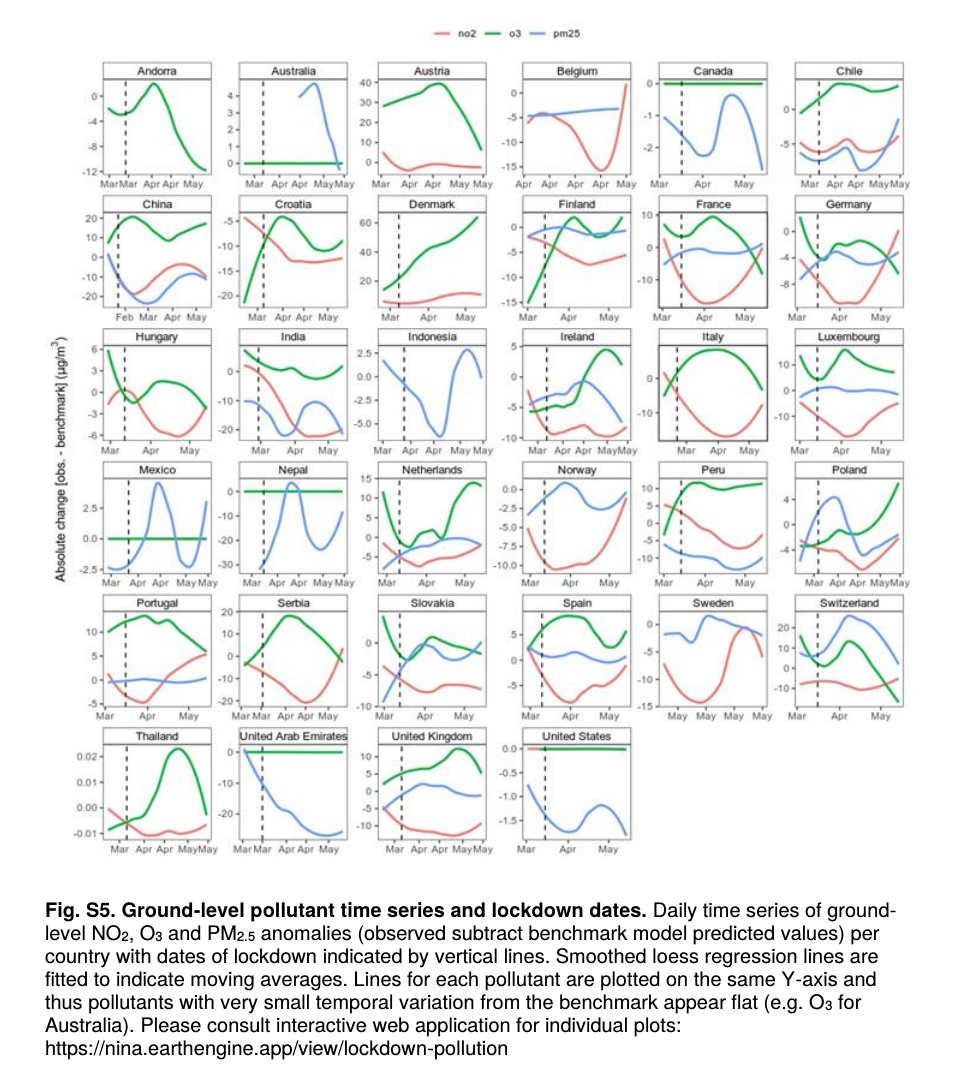
\includegraphics[width=.99\linewidth]{images/Venter2020-FigS5.png}
\caption{Ground-level pollutant time series and lockdown dates.}
 \label{fig:Venter2020}
\end{figure*} 


\section{Methods}
\subsection{Data sources}

\subsubsection{Pollution data}
The World Air Quality Index project \citep{AQICN2021} provides ground-level readings of pollutants for about 2000 cities in 132 countries sourced from world-wide environmental protection agencies. We downloaded data for about 900 cities (of the 1672 largest cities in the world\citep{UNDESA2015}) over the period 2014-2021. The pollutants downloaded were PM$_{2.5}$, PM$_{10}$, O$_{3}$, NO$_{2}$, SO$_{2}$ and CO. AQICN converts all readings from mg/m$^{3}$ to AQI levels using the EPA standard \citep{Gilliam2016} and provides a 24 hour average of hourly readings.



\subsubsection{Stringency index}

Oxford Covid-19 Government Response Tracker \citep{Hale2020} (Figure \ref{fig:oxcgrt}) daily stringency index is based on a combination of containment and closure policies and assigned an ordinal value (0 to 1, 2, 3, or 4 depending on the indicator). These include school closings, workplace closings, cancellation of public events, restrictions on gatherings, closing public transport, stay at home requirements, restrictions on internal movements, international travel controls and government public information campaigns. These are combined into an index and scaled 0-100. Each of the containment policies are also available individually. In addition, indexes are available at a state (and selected city) level for the United States and Brazil \citep{Hale2020a,Petherick2020} (Figure \ref{fig:statestr}). We downloaded the entire dataset (as of February 2021) and matched the 1672 cities to the lowest level data available (i.e. ordered by city, county/province/state, and country) in the stringency index.




\begin{figure*}
\centering
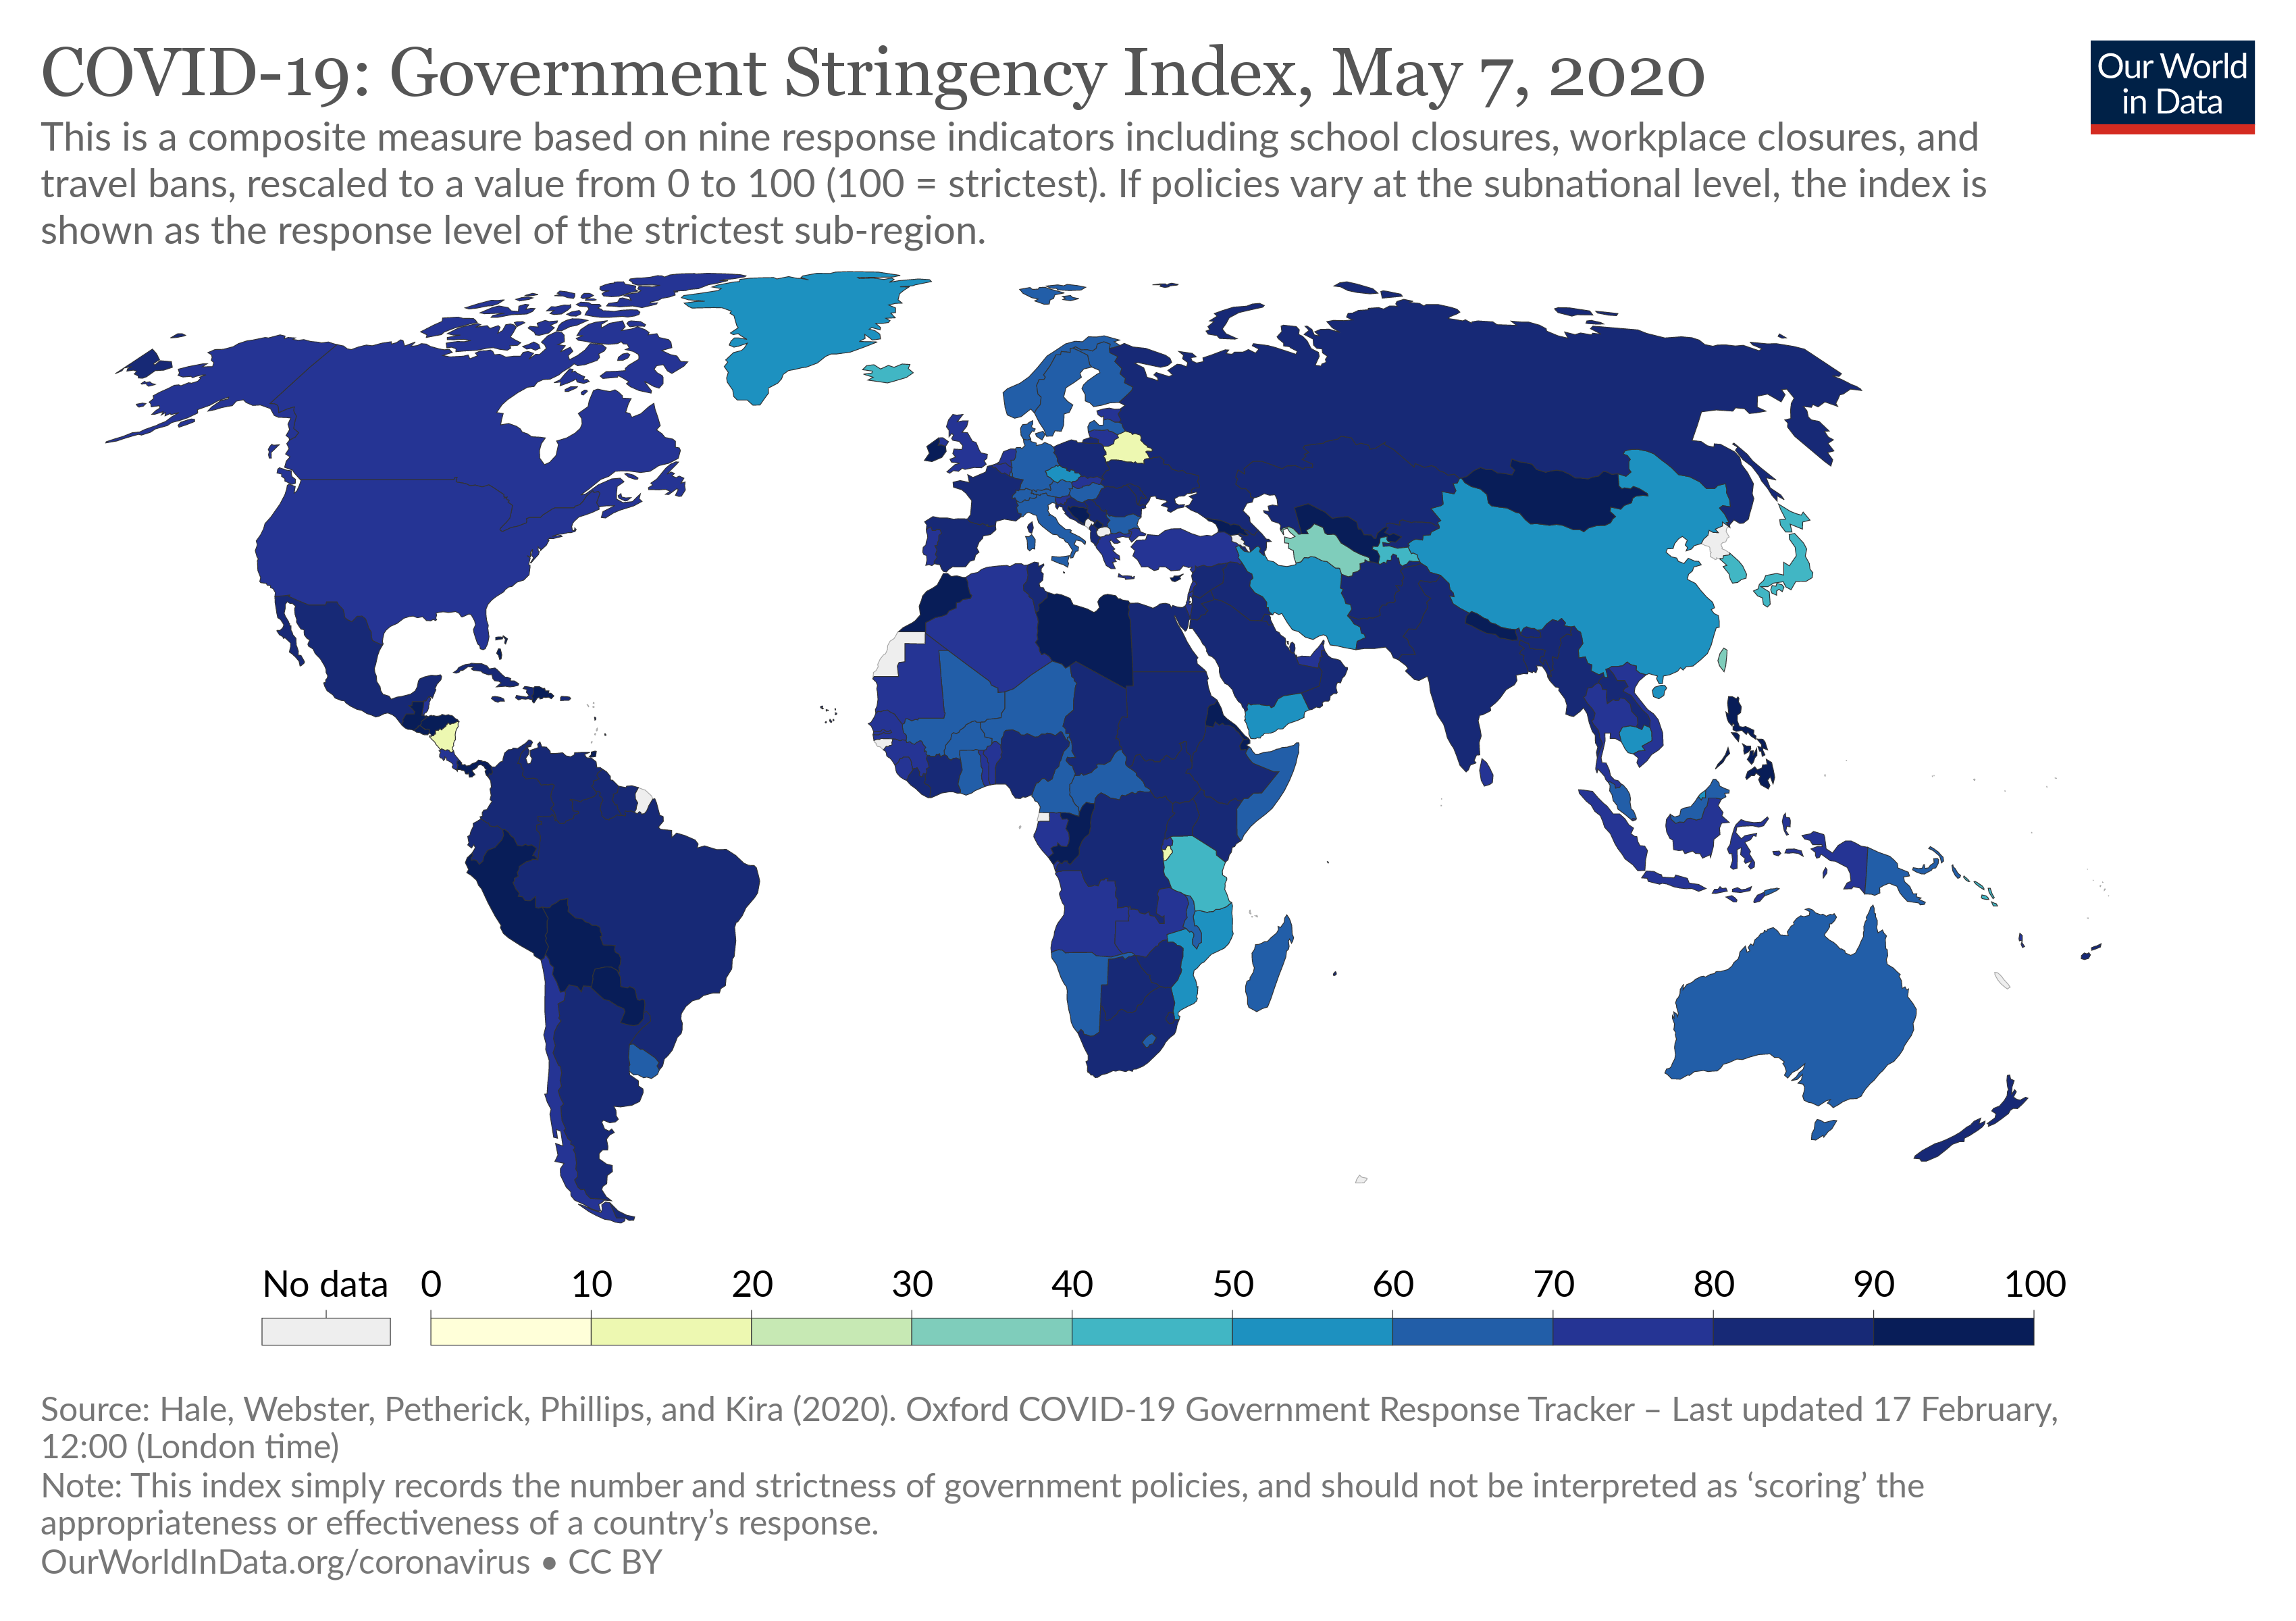
\includegraphics[width=.99\linewidth]{images/covid-stringency-index.png}
\caption{Oxford Covid-19 Government Response Tracker daily stringency index.}
 \label{fig:oxcgrt}
\end{figure*} 

\begin{figure*}
\centering
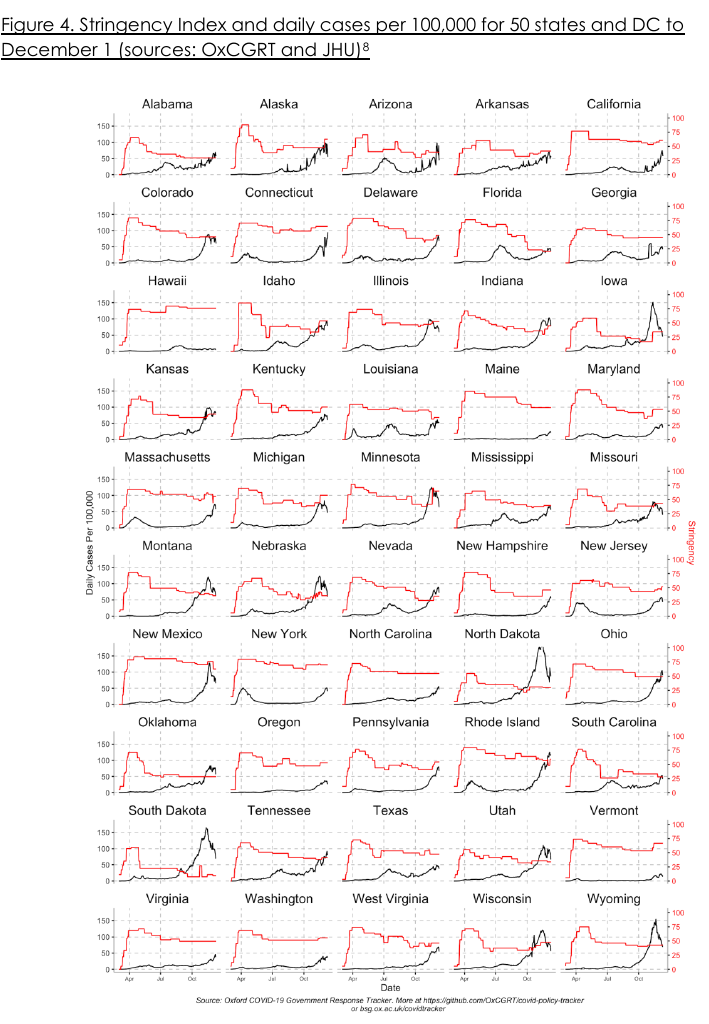
\includegraphics[width=.99\linewidth]{images/Hallas2020-stateStr.png}
\caption{Stringency index and daily cases per 100,000 for 50 states and DC to December 1\citep{Hallas2020}.}
 \label{fig:statestr}
\end{figure*}


\subsubsection{Mobility data}
\paragraph{Google}

Google COVID-19 Community Mobility Reports \citep{Google2020} provides a  daily percentage change of visitors to retail and recreation, grocery and pharmacy, parks, transit stations, workplaces, and residences from a historic baseline. The baseline is a median value from January 3 to February 6, 2020. This data is at a county/province level for all data. We mapped this data to the cities wholly included in each (i.e. Clark County for Las Vegas) or by combining multiple counties into a single city (i.e. New York City using New York, Kings, Queens, Bronx, and Richmond counties). Figure \ref{fig:googlemobility} shows mobility trends for Melbourne, Australia across 2020 and 2021.

\begin{figure*}
\centering
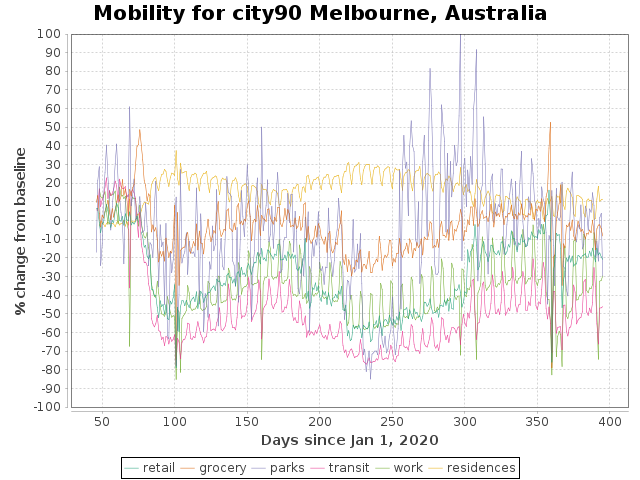
\includegraphics[width=.99\linewidth]{images/city90MelbourneAustralia.png}
\caption{Google mobility data for Melbourne, Australia across 2020 and 2021.}
 \label{fig:googlemobility}
\end{figure*}


\paragraph{Apple}
Apple Maps Mobility Trends Reports \citep{Apple2020} provides a daily percent change in Apple Maps routing requests from the baseline January 13, 2020 for driving, walking, and public transport journeys. This data is at a county/province level for all data and the mapping process was similar to the Google data. Figure \ref{fig:apple} shows mobility trends for Melbourne, Australia across 2020 and 2021.

\paragraph{Apple}
\begin{figure*}
\centering
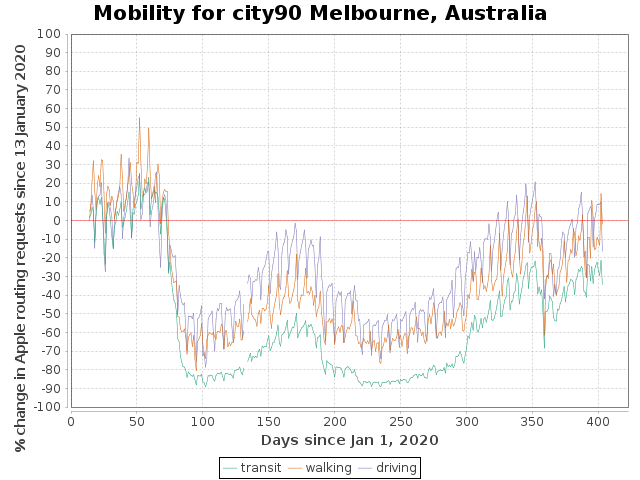
\includegraphics[width=.99\linewidth]{images/Applecity90MelbourneAustralia.png}
\caption{Apple Maps mobility data for Melbourne, Australia across 2020 and 2021.}
 \label{fig:apple}
\end{figure*}

\subsubsection{Monthly electricity statistics}
The International Energy Agency produces reports of electricity generation and usage for 47 countries for 2016-2020 \citep{IEA2021}. These reports provide a break down of monthly generation through conventional thermal and combustibles (coal, oil, natural gas, and others) and renewables (nuclear, hydro, wind, solar, and geothermal). These reports are at a country level. We mapped the country level data to each individual city. Figure \ref{fig:au-total} shows trends of Australian net electricity production from all sources 2016-2021 and trends of conventional thermal (Figure \ref{fig:au-thermal}) over the same period. Figure \ref{fig:china-net} shows Chinese electricity generation through coal 2016-2021.


\begin{figure*}
\centering
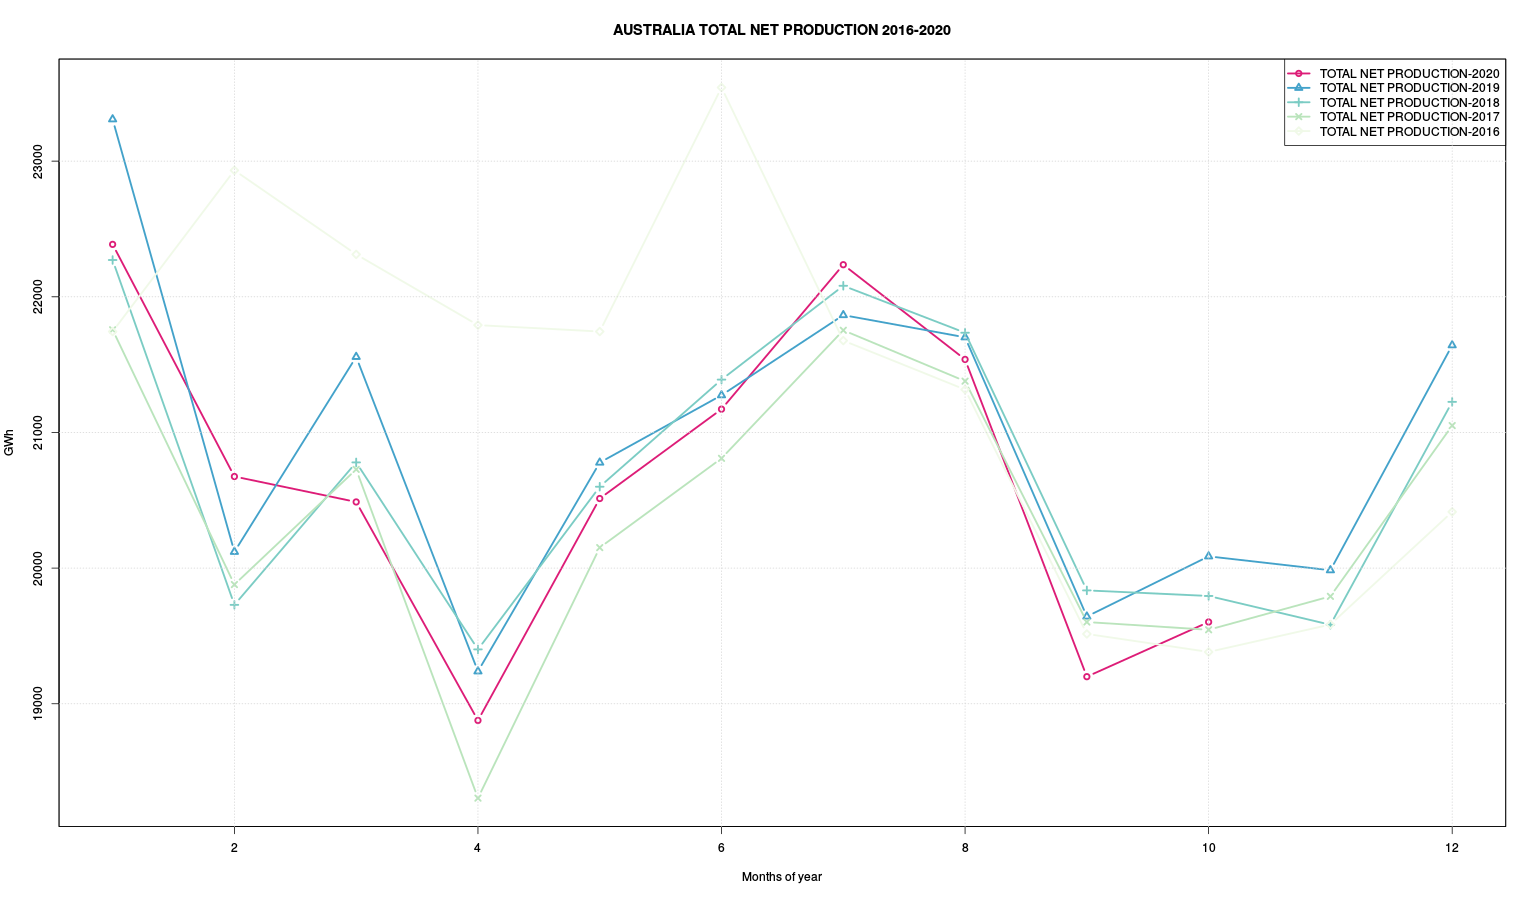
\includegraphics[width=.99\linewidth]{images/AUSTRALIATOTALNETPRODUCTION.png}
\caption{Trends of Australian net electricity production from all sources 2016-2021.}
 \label{fig:au-total}
\end{figure*}

\begin{figure*}
\centering
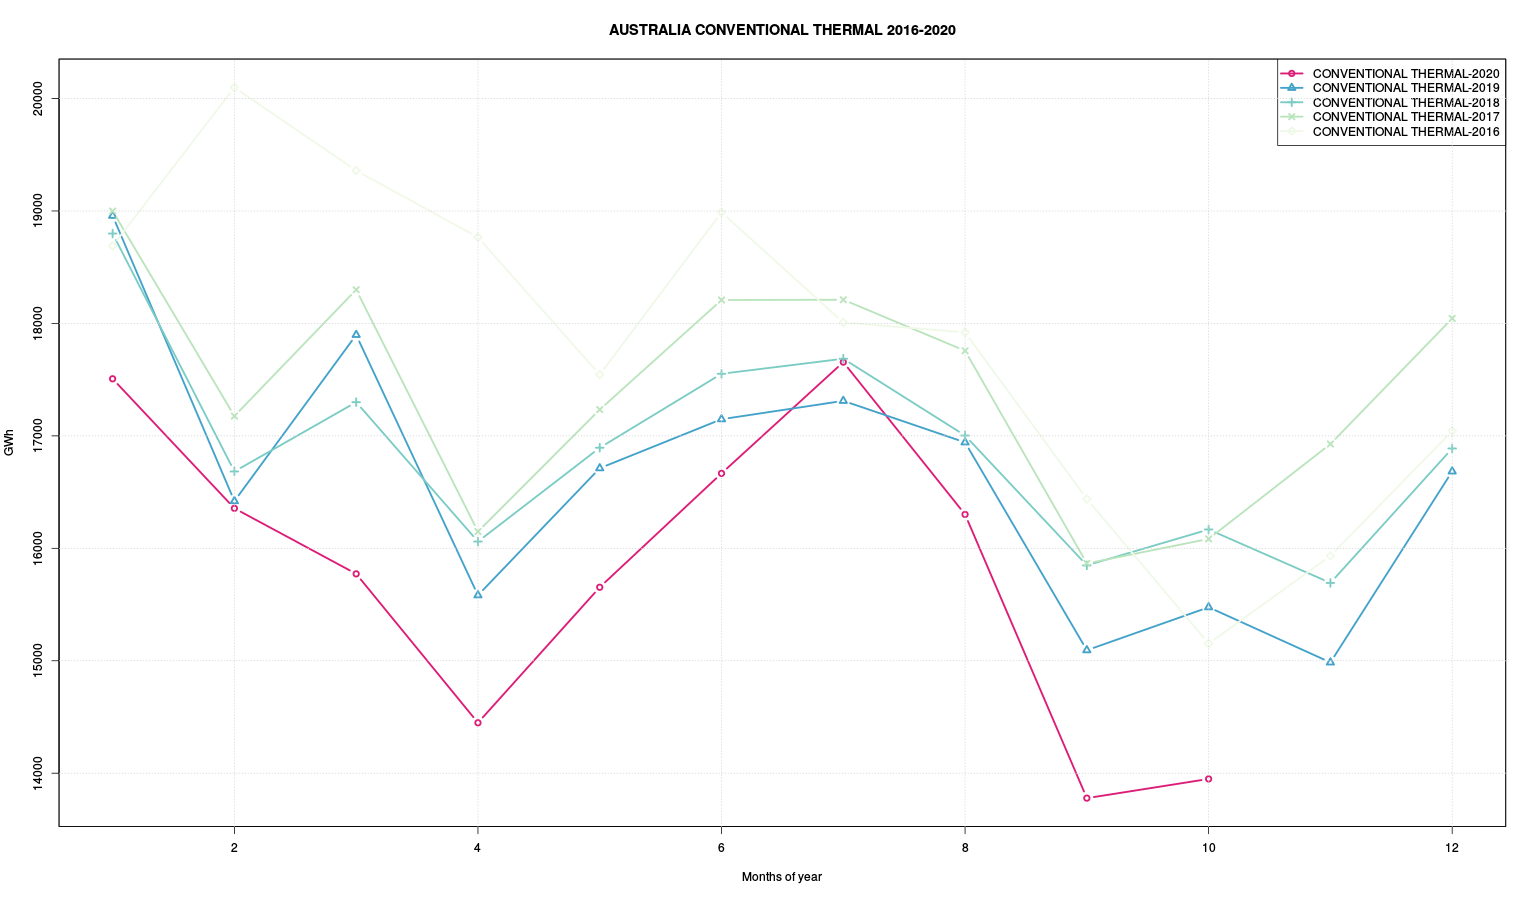
\includegraphics[width=.99\linewidth]{images/AUSTRALIACONVENTIONALTHERMAL.png}
\caption{Trends of Australian electricity production from conventional thermal 2016-2021.}
 \label{fig:au-thermal}
\end{figure*}

\begin{figure*}
\centering
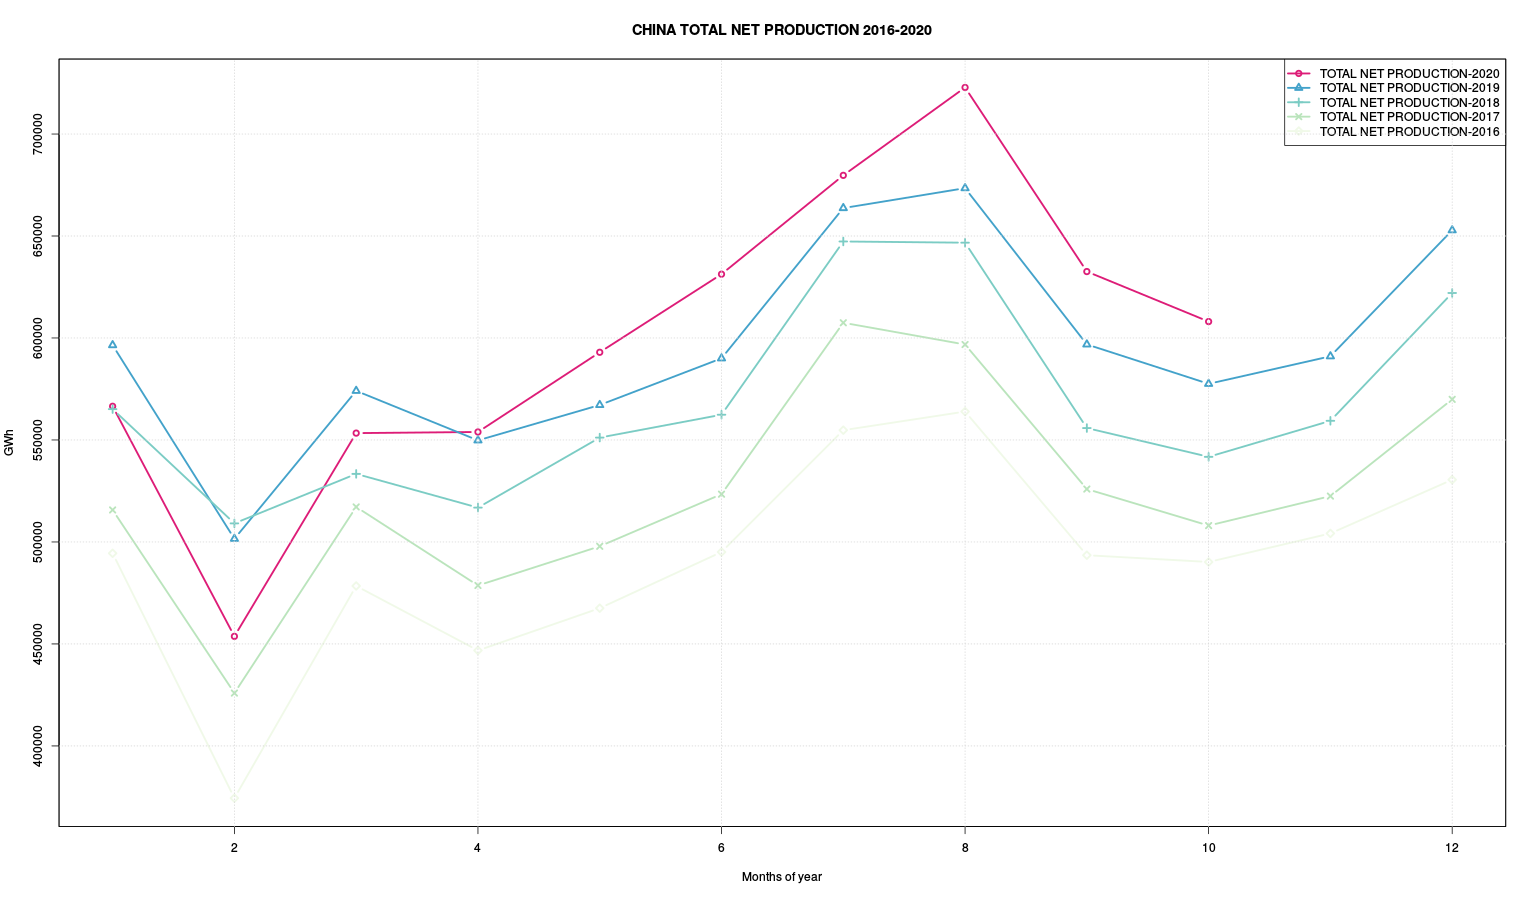
\includegraphics[width=.99\linewidth]{images/CHINATOTALNETPRODUCTION.png}
\caption{Trends of Chinese electricity production from coal 2016-2021.}
 \label{fig:china-net}
\end{figure*}


\section*{References}\label{sec:ref}

  \bibliographystyle{elsarticle-harv} 
 % \bibliography{bib}
   \bibliography{COVID.bib}


\end{document}
